\chapter{表格、表单}

\section{table标签}

\subsection{table标签}

有时候需要在网页中添加一些表格数据,如企业员工通讯录等。

\begin{figure}[H]
    \centering
    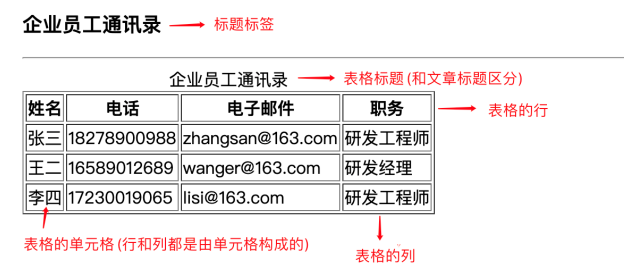
\includegraphics[scale=0.9]{img/C4/4-1/1.png}
    \caption{企业员工通讯录}
\end{figure}

创建表格主要包含5个元素:

\begin{enumerate}
    \item \lstinline|<caption>|:定义表格的标题。

    \item \lstinline|<table>|:整个表格以\lstinline|<table>|开始、\lstinline|</table>|结束,\lstinline|<table>|在没有添加border属性之前,在浏览器中显示是没有表格线的。

    \item \lstinline|<tr>|:表格的一行,有几对\lstinline|<tr>|表格就有几行,\lstinline|<tr>|里只能放\lstinline|<th>|或者\lstinline|<td>|。

    \item \lstinline|<th>|:表格头部的一个单元格,会加粗居中显示。

    \item \lstinline|<td>|:表格的一个单元格,有几对\lstinline|<td>|一行中就有几列。
\end{enumerate}

\begin{lstlisting}[style=htmlcssjs, title=企业员工通讯录]
<!DOCTYPE html>
<html lang="en">
<head>
    <meta charset="UTF-8">
    <title>企业员工通讯录</title>
</head>
<body>
    <h3>企业员工通讯录</h3>
    <hr/>

    <!-- 表格标签 border属性代表给表格加上边框 -->
    <table border="1">
        <!-- 表格标题 -->
        <caption>企业员工通讯录</caption>
        <!-- tr代表一行 -->
        <tr>
            <!-- th代表表格头部的一个单元格 -->
            <th>姓名</th>
            <th>电话</th>
            <th>电子邮件</th>
            <th>职务</th>
        </tr>
        <tr>
            <!-- td代表一个单元格 -->
            <td>张三</td>
            <td>18278900988</td>
            <td>zhangsan@163.com</td>
            <td>研发工程师</td>
        </tr>
        <tr>
            <td>王二</td>
            <td>16589012689</td>
            <td>wanger@163.com</td>
            <td>研发经理</td>
        </tr>
        <tr>
            <td>李四</td>
            <td>17230019065</td>
            <td>lisi@163.com</td>
            <td>研发工程师</td>
        </tr>
    </table>
</body>
</html>
\end{lstlisting}

\newpage

\section{与用户交互——form标签}

\subsection{form标签}

使用HTML表单(form)可以实现网站与用户的交互,表单可以把浏览者输入的数据传送到服务器端,这样服务器端程序就可以处理表单传过来的数据。 \\

\begin{lstlisting}[style=htmlcssjs]
<form method="传送方式" action="服务器文件">表单内容</form>
\end{lstlisting}

\lstinline|<form>|是成对出现的,以\lstinline|<form>|开始、\lstinline|</form>|结束。method属性表示数据传送的方式,包括get和post两种方式,get和post的区别属于后端程序员需要考虑的问题,完全取决于后端人员要求什么方式进行传输。action属性表示浏览者输入的数据被传送到的地方,比如一个PHP页面。 \\

所有的表单控件(文本框、文本域、按钮、单选框、复选框等)都必须放在\lstinline|<form>|之间,否则用户输入的信息无法提交到服务器上。

\newpage

\section{先来填用户名和密码——文本、密码输入框}

\subsection{文本、密码输入框}

当用户需要在表单中输入字母、数字等内容时,就需要使用到文本输入框,文本框也可转化为密码输入框。 \\

\begin{lstlisting}[style=htmlcssjs]
<form>
    <input type="text/password" name="名称" value="文本" />
</form>
<form>
    <input type="text/password" name="名称" value="文本" />
</form>
\end{lstlisting}

\begin{itemize}
    \item \lstinline|type="text"|:输入框为文本输入框
    \item \lstinline|type="password"|:输入框为密码输入框
    \item name:为文本框命名,以备后台程序使用
    \item value:为文本输入框设置默认值,一般起提示作用
\end{itemize}

\subsection{给点提示呗——placeholder属性}

有时候需要提示用户输入框需要输入的内容,这时候就需要使用\lstinline|<input>|中的占位符placeholder属性。

\begin{figure}[H]
    \centering
    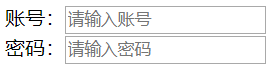
\includegraphics[]{img/C4/4-3/1.png}
    \caption{placeholder提示文本}
\end{figure}

placeholder属性的值可以根据情况合理填写,当输入框输入内容时,占位符内容消失,当输入框无内容时,占位符内容显示。注意,占位符内容不是输入框真正的内容。

\subsection{重置按钮}

当用户需要重置表单信息到初始状态时,比如输入“账号”或“密码”有误,就可以使用重置按钮使输入框恢复到初始状态。通过设置\lstinline|<input>|中type属性为reset即可实现重置按钮。

\subsection{提交按钮}

当用户需要提交表单信息到服务器时,需要用到提交按钮。通过设置\lstinline|<input>|中type属性为submit即可实现提交按钮。表单信息会被发送给后端,在数据库对比账户和密码信息。

\begin{lstlisting}[style=htmlcssjs, title=登录功能]
<!DOCTYPE html>
<html lang="en">
<head>
    <meta charset="UTF-8">
    <title>登录</title>
</head>
<body>
    <form action="get/post">
        账号:<input type="text" placeholder="请输入账号" name="username">
        <br/>
        密码:<input type="password" placeholder="请输入密码" name="password">
        <br/>
        <input type="submit">
        <input type="reset">
    </form>
</body>
</html>
\end{lstlisting}

\newpage

\section{数字、网址、邮箱输入框}

\subsection{数字输入框}

将\lstinline|<input>|的type属性设置为number,则表示该输入框的类型为数字。数字框只能输入数字,输入其它字符无效。数字框最右侧会有一个加减符号,可以调整输入数字的大小,不同浏览器表现不一致。

\subsection{网址输入框}

将\lstinline|<input>|的type属性设置为url,则表示输入类型为网址。网址输入框必须以http://或https://开头,且后面必须有内容,否则表单提交的时候会报错误提示。

\subsection{邮箱输入框}

将\lstinline|<input>|的type属性设置为email,则表示该输入框的类型为邮箱。邮箱输入框的值必须包含`@`,并且之后必须有内容,否则会报错误提示。

\begin{lstlisting}[style=htmlcssjs, title=个人信息]
<!DOCTYPE html>
<html lang="en">
<head>
    <meta charset="UTF-8">
    <title>个人信息</title>
</head>
<body>
    <form action="get/post">
        姓名:<input type="text" name="name"><br/>
        年龄:<input type="number" name="age"><br/>
        主页:<input type="url" name="webpage"><br/>
        邮箱:<input type="email" name="email"><br/>
        <input type="submit">
        <input type="reset">
    </form>
</body>
</html>
\end{lstlisting}

\newpage

\section{文本域}

\subsection{文本域}

当用户需要在表单中输入大段文字时,就需要用到文本输入域。\lstinline|<textarea>|中也可以设置placeholder属性来显示提示信息。 \\

\begin{lstlisting}[style=htmlcssjs]
<textarea rows="行数" cols="列数">文本</textarea>
\end{lstlisting}

\begin{itemize}
    \item rows:多行输入域的行数,可以用CSS样式的height代替
    \item cols:多行输入域的列数,可以用CSS样式的width代替
\end{itemize}

\begin{lstlisting}[style=htmlcssjs, title=文本域]
<!DOCTYPE html>
<html lang="en">
<head>
    <meta charset="UTF-8">
    <title>文本域</title>
</head>
<body>
    <form action="get/post">
        <textarea cols="30" rows="10" placeholder="请输入..."></textarea>
    </form>
</body>
</html>
\end{lstlisting}

\newpage

\section{label标签}

\subsection{label标签}

\lstinline|<label>|不会向用户呈现任何特殊特效,它的作用是为鼠标用户改进了可用性。如果在\lstinline|<label>|内点击文本,就会触发此控件。也就是说,当用户单击选中该\lstinline|<label>|时,浏览器就会自动将焦点转到和标签相关的表单控件上。

\begin{lstlisting}[style=htmlcssjs]
<label for="控件id名称">
\end{lstlisting}

注意,\lstinline|<label>|的for属性的值必须要与相关空间的id属性值相同。

\begin{lstlisting}[style=htmlcssjs, title=label标签]
<!DOCTYPE html>
<html lang="en">
<head>
    <meta charset="UTF-8">
    <title>label标签</title>
</head>
<body>
    <form action="get/post">
        <label for="username">用户名:</label>
        <input type="text" id="username">
    </form>
</body>
</html>
\end{lstlisting}

\newpage

\section{单选框、复选框}

\subsection{单选框、复选框}

在使用表单设计调查表时,为了减少用户的操作,使用选择框是一个好主意。HTML中有两种选择框,即单选框和复选框,两者的区别是单选框中的选项用户只能选择一项,而复选框中用户可以任意选择多项,甚至全选。 \\

\begin{lstlisting}[style=htmlcssjs]
<input type="radio/checkbox" name="名称" value="值" checked="checked">
\end{lstlisting}

\begin{itemize}
    \item \lstinline|type="radio"|:单选框
    \item \lstinline|type="checkbox"|:复选框
    \item name:为控件命名,具有相同名称的选择框属于同一组
    \item checked:设置默认选中的值
\end{itemize}

在网页开发中,往往需要优化用户体验。一个好的产品有3个特点:解决刚需的问题、用户体验、用户黏性(产品定位)。用户体验就是养成用户的懒习惯,减少用户操作,能不让用户操作就不让用户操作,节省用户时间,用户不动手就会觉得方便。例如一个选择性别的单选框,概率上看,假设有100个人,50男50女,使用默认选项,可以节省一半人的操作。

\begin{lstlisting}[style=htmlcssjs, title=单选框/复选框]
<!DOCTYPE html>
<html lang="en">
<head>
    <meta charset="UTF-8">
    <title>单选框/复选框</title>
</head>
<body>
    <form action="get/post">
        1. 您是否喜欢运动?
        <input type="radio" name="sport" checked="checked">是
        <input type="radio" name="sport">否
        2. 您喜欢的运动是?
        <input type="checkbox" name="sport_item">跑步
        <input type="checkbox" name="sport_item">篮球
        <input type="checkbox" name="sport_item">羽毛球
    </form>
</body>
</html>
\end{lstlisting}

\newpage

\section{下拉列表}

\subsection{下拉列表}

下拉列表在网页中也常会用到,它可以有效的节省网页空间。下拉列表既可以单选也可以多选。 \\

\begin{lstlisting}[style=htmlcssjs]
<select>
    <option value="值">选项</option>
    <option value="值">选项</option>
</select>
\end{lstlisting}

\begin{itemize}
    \item value:向服务器提交的值,而双标签中间的内容才是显示的值
    \item selected:设置\lstinline|selected="selected"|表示该选项被默认选中
\end{itemize}

\begin{lstlisting}[style=htmlcssjs, title=下拉列表]
<!DOCTYPE html>
<html lang="en">
<head>
    <meta charset="UTF-8">
    <title>下拉列表</title>
</head>
<body>
    <form action="get/post">
        <select>
            <option value="male" selected="selected">男</option>
            <option value="female">女</option>
        </select>
    </form>
</body>
</html>
\end{lstlisting}

\newpage